% Created by tikzDevice version 0.12.3 on 2020-04-21 11:12:11
% !TEX encoding = UTF-8 Unicode
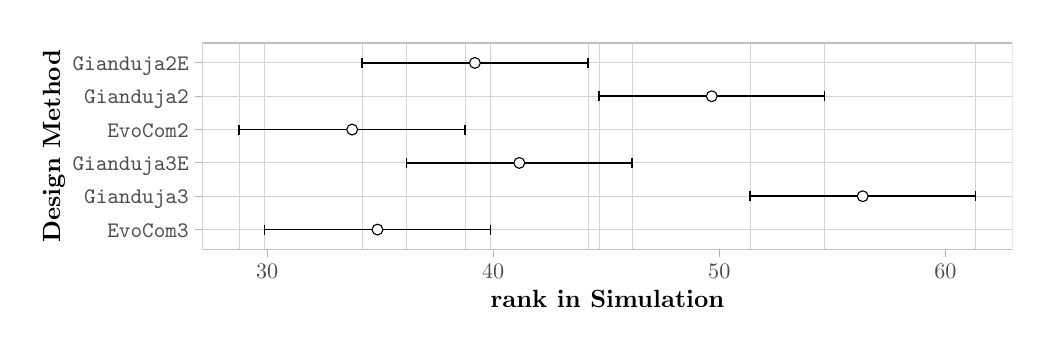
\begin{tikzpicture}[x=1pt,y=1pt]
\definecolor{fillColor}{RGB}{255,255,255}
\path[use as bounding box,fill=fillColor,fill opacity=0.00] (0,0) rectangle (361.35,108.41);
\begin{scope}
\path[clip] (  0.00,  0.00) rectangle (361.35,108.41);
\definecolor{drawColor}{RGB}{255,255,255}
\definecolor{fillColor}{RGB}{255,255,255}

\path[draw=drawColor,line width= 0.6pt,line join=round,line cap=round,fill=fillColor] (  0.00,  0.00) rectangle (361.35,108.41);
\end{scope}
\begin{scope}
\path[clip] ( 63.15, 28.23) rectangle (355.85,102.91);
\definecolor{fillColor}{RGB}{255,255,255}

\path[fill=fillColor] ( 63.15, 28.23) rectangle (355.85,102.91);
\definecolor{drawColor}{RGB}{211,211,211}

\path[draw=drawColor,line width= 0.3pt,line join=round] ( 63.15, 71.59) --
	(355.85, 71.59);

\path[draw=drawColor,line width= 0.3pt,line join=round] ( 63.15, 35.45) --
	(355.85, 35.45);

\path[draw=drawColor,line width= 0.3pt,line join=round] ( 63.15, 83.63) --
	(355.85, 83.63);

\path[draw=drawColor,line width= 0.3pt,line join=round] ( 63.15, 95.68) --
	(355.85, 95.68);

\path[draw=drawColor,line width= 0.3pt,line join=round] ( 63.15, 47.50) --
	(355.85, 47.50);

\path[draw=drawColor,line width= 0.3pt,line join=round] ( 63.15, 59.54) --
	(355.85, 59.54);

\path[draw=drawColor,line width= 0.2pt,line join=round] (158.05, 28.23) -- (158.05,102.91);

\path[draw=drawColor,line width= 0.2pt,line join=round] (167.20, 28.23) -- (167.20,102.91);

\path[draw=drawColor,line width= 0.2pt,line join=round] (287.99, 28.23) -- (287.99,102.91);

\path[draw=drawColor,line width= 0.2pt,line join=round] (202.40, 28.23) -- (202.40,102.91);

\path[draw=drawColor,line width= 0.2pt,line join=round] (342.55, 28.23) -- (342.55,102.91);

\path[draw=drawColor,line width= 0.2pt,line join=round] (218.45, 28.23) -- (218.45,102.91);

\path[draw=drawColor,line width= 0.2pt,line join=round] ( 76.45, 28.23) -- ( 76.45,102.91);

\path[draw=drawColor,line width= 0.2pt,line join=round] ( 85.60, 28.23) -- ( 85.60,102.91);

\path[draw=drawColor,line width= 0.2pt,line join=round] (206.39, 28.23) -- (206.39,102.91);

\path[draw=drawColor,line width= 0.2pt,line join=round] (120.80, 28.23) -- (120.80,102.91);

\path[draw=drawColor,line width= 0.2pt,line join=round] (260.95, 28.23) -- (260.95,102.91);

\path[draw=drawColor,line width= 0.2pt,line join=round] (136.85, 28.23) -- (136.85,102.91);
\definecolor{drawColor}{RGB}{0,0,0}

\path[draw=drawColor,line width= 0.6pt,line join=round] (158.05, 69.78) --
	(158.05, 73.39);

\path[draw=drawColor,line width= 0.6pt,line join=round] (158.05, 71.59) --
	( 76.45, 71.59);

\path[draw=drawColor,line width= 0.6pt,line join=round] ( 76.45, 69.78) --
	( 76.45, 73.39);

\path[draw=drawColor,line width= 0.6pt,line join=round] (167.20, 33.65) --
	(167.20, 37.26);

\path[draw=drawColor,line width= 0.6pt,line join=round] (167.20, 35.45) --
	( 85.60, 35.45);

\path[draw=drawColor,line width= 0.6pt,line join=round] ( 85.60, 33.65) --
	( 85.60, 37.26);

\path[draw=drawColor,line width= 0.6pt,line join=round] (287.99, 81.83) --
	(287.99, 85.44);

\path[draw=drawColor,line width= 0.6pt,line join=round] (287.99, 83.63) --
	(206.39, 83.63);

\path[draw=drawColor,line width= 0.6pt,line join=round] (206.39, 81.83) --
	(206.39, 85.44);

\path[draw=drawColor,line width= 0.6pt,line join=round] (202.40, 93.87) --
	(202.40, 97.48);

\path[draw=drawColor,line width= 0.6pt,line join=round] (202.40, 95.68) --
	(120.80, 95.68);

\path[draw=drawColor,line width= 0.6pt,line join=round] (120.80, 93.87) --
	(120.80, 97.48);

\path[draw=drawColor,line width= 0.6pt,line join=round] (342.55, 45.69) --
	(342.55, 49.30);

\path[draw=drawColor,line width= 0.6pt,line join=round] (342.55, 47.50) --
	(260.95, 47.50);

\path[draw=drawColor,line width= 0.6pt,line join=round] (260.95, 45.69) --
	(260.95, 49.30);

\path[draw=drawColor,line width= 0.6pt,line join=round] (218.45, 57.74) --
	(218.45, 61.35);

\path[draw=drawColor,line width= 0.6pt,line join=round] (218.45, 59.54) --
	(136.85, 59.54);

\path[draw=drawColor,line width= 0.6pt,line join=round] (136.85, 57.74) --
	(136.85, 61.35);

\path[draw=drawColor,line width= 0.4pt,line join=round,line cap=round,fill=fillColor] (117.25, 71.59) circle (  1.96);

\path[draw=drawColor,line width= 0.4pt,line join=round,line cap=round,fill=fillColor] (126.40, 35.45) circle (  1.96);

\path[draw=drawColor,line width= 0.4pt,line join=round,line cap=round,fill=fillColor] (247.19, 83.63) circle (  1.96);

\path[draw=drawColor,line width= 0.4pt,line join=round,line cap=round,fill=fillColor] (161.60, 95.68) circle (  1.96);

\path[draw=drawColor,line width= 0.4pt,line join=round,line cap=round,fill=fillColor] (301.75, 47.50) circle (  1.96);

\path[draw=drawColor,line width= 0.4pt,line join=round,line cap=round,fill=fillColor] (177.65, 59.54) circle (  1.96);
\definecolor{drawColor}{RGB}{190,190,190}

\path[draw=drawColor,line width= 0.6pt,line join=round,line cap=round] ( 63.15, 28.23) rectangle (355.85,102.91);
\end{scope}
\begin{scope}
\path[clip] (  0.00,  0.00) rectangle (361.35,108.41);
\definecolor{drawColor}{gray}{0.30}

\node[text=drawColor,anchor=base east,inner sep=0pt, outer sep=0pt, scale=  0.80] at ( 58.20, 68.83) {\texttt{EvoCom2}};

\node[text=drawColor,anchor=base east,inner sep=0pt, outer sep=0pt, scale=  0.80] at ( 58.20, 32.70) {\texttt{EvoCom3}};

\node[text=drawColor,anchor=base east,inner sep=0pt, outer sep=0pt, scale=  0.80] at ( 58.20, 80.88) {\texttt{Gianduja2}};

\node[text=drawColor,anchor=base east,inner sep=0pt, outer sep=0pt, scale=  0.80] at ( 58.20, 92.92) {\texttt{Gianduja2E}};

\node[text=drawColor,anchor=base east,inner sep=0pt, outer sep=0pt, scale=  0.80] at ( 58.20, 44.74) {\texttt{Gianduja3}};

\node[text=drawColor,anchor=base east,inner sep=0pt, outer sep=0pt, scale=  0.80] at ( 58.20, 56.79) {\texttt{Gianduja3E}};
\end{scope}
\begin{scope}
\path[clip] (  0.00,  0.00) rectangle (361.35,108.41);
\definecolor{drawColor}{gray}{0.70}

\path[draw=drawColor,line width= 0.3pt,line join=round] ( 60.40, 71.59) --
	( 63.15, 71.59);

\path[draw=drawColor,line width= 0.3pt,line join=round] ( 60.40, 35.45) --
	( 63.15, 35.45);

\path[draw=drawColor,line width= 0.3pt,line join=round] ( 60.40, 83.63) --
	( 63.15, 83.63);

\path[draw=drawColor,line width= 0.3pt,line join=round] ( 60.40, 95.68) --
	( 63.15, 95.68);

\path[draw=drawColor,line width= 0.3pt,line join=round] ( 60.40, 47.50) --
	( 63.15, 47.50);

\path[draw=drawColor,line width= 0.3pt,line join=round] ( 60.40, 59.54) --
	( 63.15, 59.54);
\end{scope}
\begin{scope}
\path[clip] (  0.00,  0.00) rectangle (361.35,108.41);
\definecolor{drawColor}{gray}{0.70}

\path[draw=drawColor,line width= 0.3pt,line join=round] ( 86.52, 25.48) --
	( 86.52, 28.23);

\path[draw=drawColor,line width= 0.3pt,line join=round] (168.22, 25.48) --
	(168.22, 28.23);

\path[draw=drawColor,line width= 0.3pt,line join=round] (249.91, 25.48) --
	(249.91, 28.23);

\path[draw=drawColor,line width= 0.3pt,line join=round] (331.60, 25.48) --
	(331.60, 28.23);
\end{scope}
\begin{scope}
\path[clip] (  0.00,  0.00) rectangle (361.35,108.41);
\definecolor{drawColor}{gray}{0.30}

\node[text=drawColor,anchor=base,inner sep=0pt, outer sep=0pt, scale=  0.80] at ( 86.52, 17.77) {30};

\node[text=drawColor,anchor=base,inner sep=0pt, outer sep=0pt, scale=  0.80] at (168.22, 17.77) {40};

\node[text=drawColor,anchor=base,inner sep=0pt, outer sep=0pt, scale=  0.80] at (249.91, 17.77) {50};

\node[text=drawColor,anchor=base,inner sep=0pt, outer sep=0pt, scale=  0.80] at (331.60, 17.77) {60};
\end{scope}
\begin{scope}
\path[clip] (  0.00,  0.00) rectangle (361.35,108.41);
\definecolor{drawColor}{RGB}{0,0,0}

\node[text=drawColor,anchor=base,inner sep=0pt, outer sep=0pt, scale=  0.90] at (209.50,  7.25) {\bfseries rank in Simulation};
\end{scope}
\begin{scope}
\path[clip] (  0.00,  0.00) rectangle (361.35,108.41);
\definecolor{drawColor}{RGB}{0,0,0}

\node[text=drawColor,rotate= 90.00,anchor=base,inner sep=0pt, outer sep=0pt, scale=  0.90] at ( 11.71, 65.57) {\bfseries Design Method};
\end{scope}
\end{tikzpicture}
